\documentclass[11pt,a4paper]{article}
\usepackage[margin=0.8in]{geometry}
\usepackage{pdfpages}

\title{\textbf{PrismSpace System Architecture \& Machine Learning Diagrams}}
\author{\textbf{Multi-Agent Swarm, ML Intelligence Routing, \& IndexedDB Architecture}}
\date{}

\begin{document}

\maketitle
\thispagestyle{empty}

\begin{abstract}
This document compiles the complete architectural specification diagrams for \textbf{PrismSpace}, including:
\begin{enumerate}
    \item \textbf{Figure 4.1: Framework of PrismSpace Multi-Agent System} --- Heterogeneous dataset ingestion, curated sources, feature engineering, swarm graph representation $\mathcal{G}(V, E)$, and the multi-model intelligence prediction pipeline with skip-connections.
    \item \textbf{Figure 4.2: Architecture Work Flow (Different Layers)} --- Layered operational architecture spanning the Presentation Layer (Next.js React 19 UI), API Bridge \& Gateway Layer (FastAPI Hive Bridge), Feature \& Routing Layer (TF-IDF + XGBoost), Multi-Agent Orchestration \& ReAct Layer (DAG Planner + MCP Tools), Evaluation \& Safety Layer (Approval Gate + ORPO Reward), and Deployment \& Storage Layer.
    \item \textbf{Figure 4.3: Overall End-to-End System Flow} --- Sequential pipeline tracing user objectives through preprocessing, feature vectorization, anomaly detection, multi-model intelligence, DAG generation, ReAct execution, SSE streaming, and persistent storage.
    \item \textbf{Figure 4.4: Browser IndexedDB Architecture \& Database Schema (\texttt{PrismDB})} --- Client-side reactive data bridge (\texttt{useLiveQuery}), Dexie.js v3 database engine, and relational entity schemas across multi-agent chat, task management, habit tracking, focus sessions, and configuration stores.
    \item \textbf{Section 4.5: Algorithm of PrismSpace Multi-Agent System} --- Formal mathematical and operational algorithmic specification: input/output definitions, data preprocessing, Pearson swarm graph construction, GAT attention-based message passing, multi-task classification, Odds Ratio Preference Optimization (\textbf{ORPO}) reward alignment, real-time runtime inference and UI generation (Next.js query capture, DAG scheduling, ReAct MCP tool execution, ORPO safety gating, SSE streaming, and Dexie IndexedDB persistence), model evaluation metrics, and workflow interpretation.
\end{enumerate}
\end{abstract}

\newpage
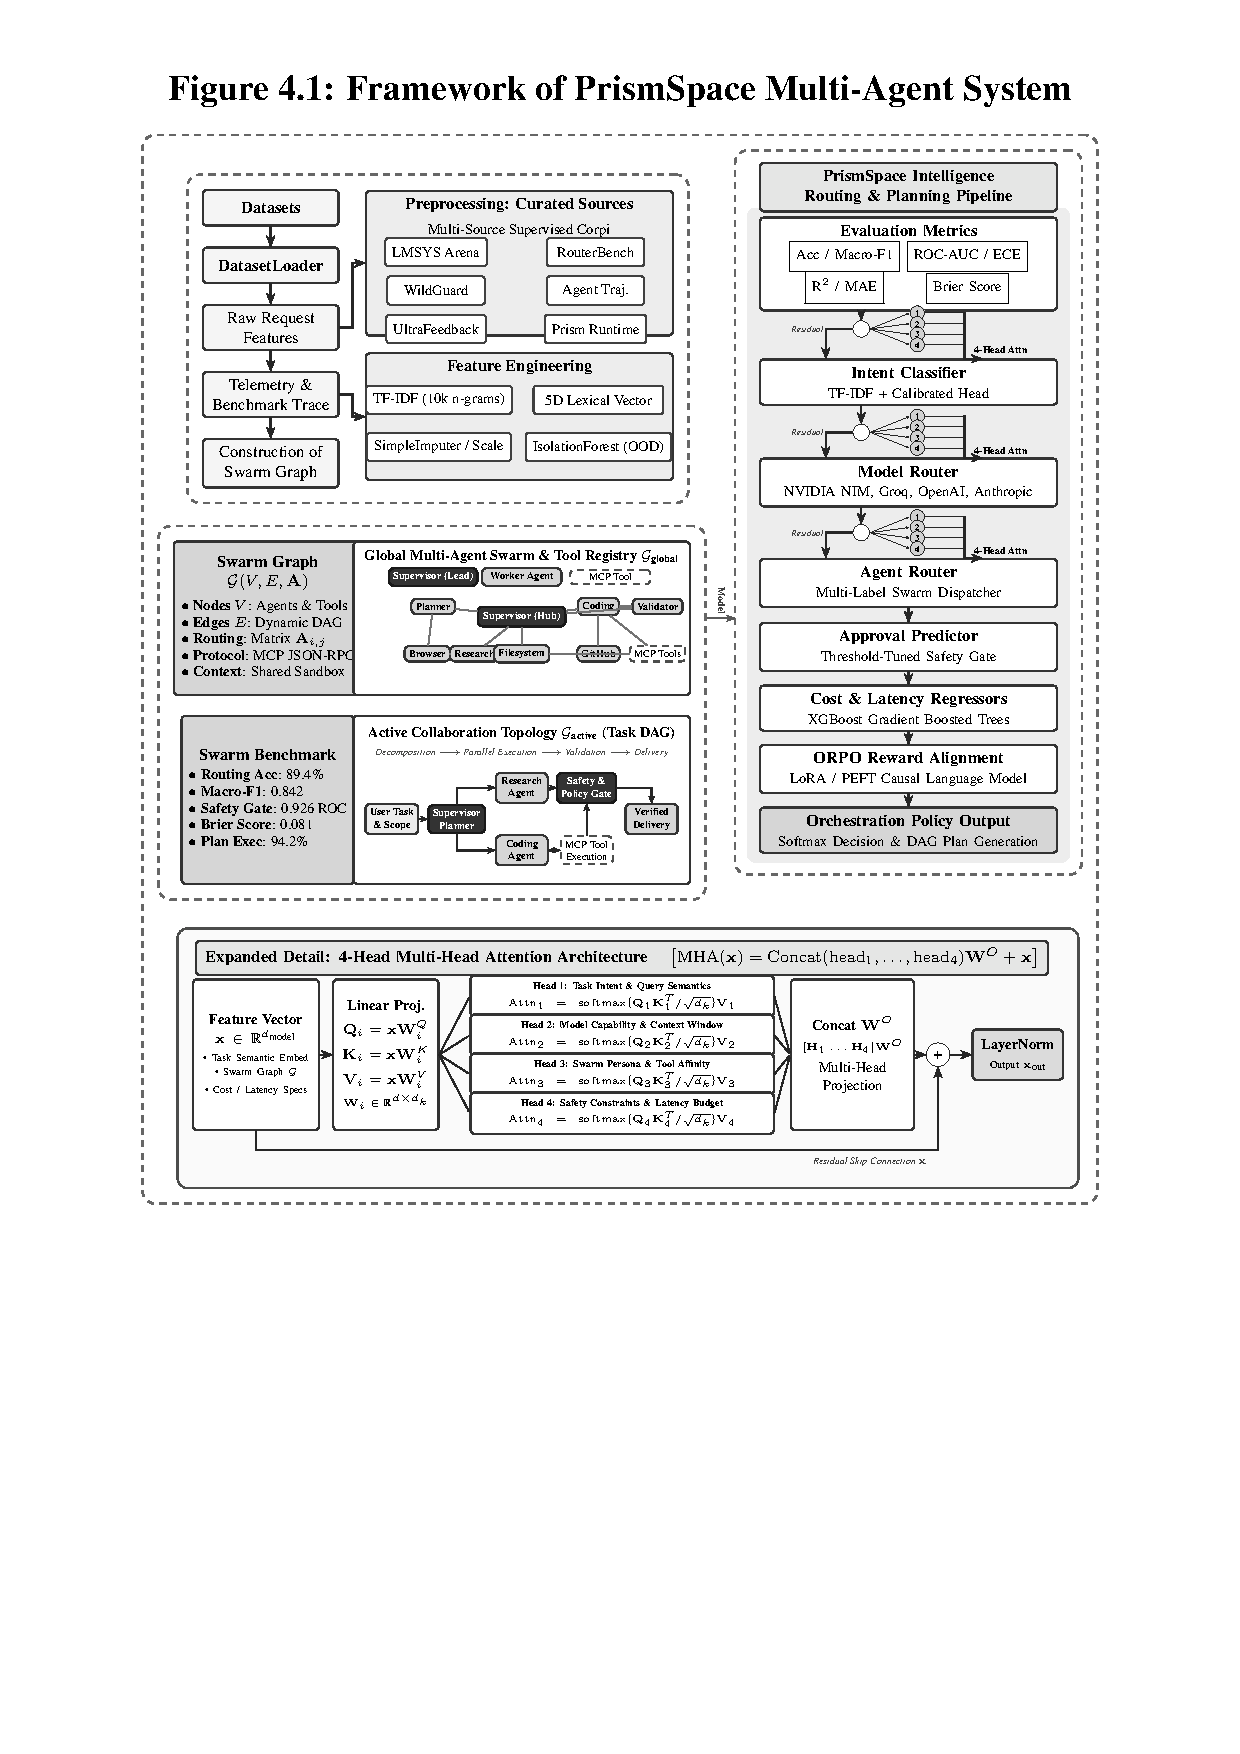
\includepdf[pages=1, fitpaper=true]{framework.pdf}

\newpage
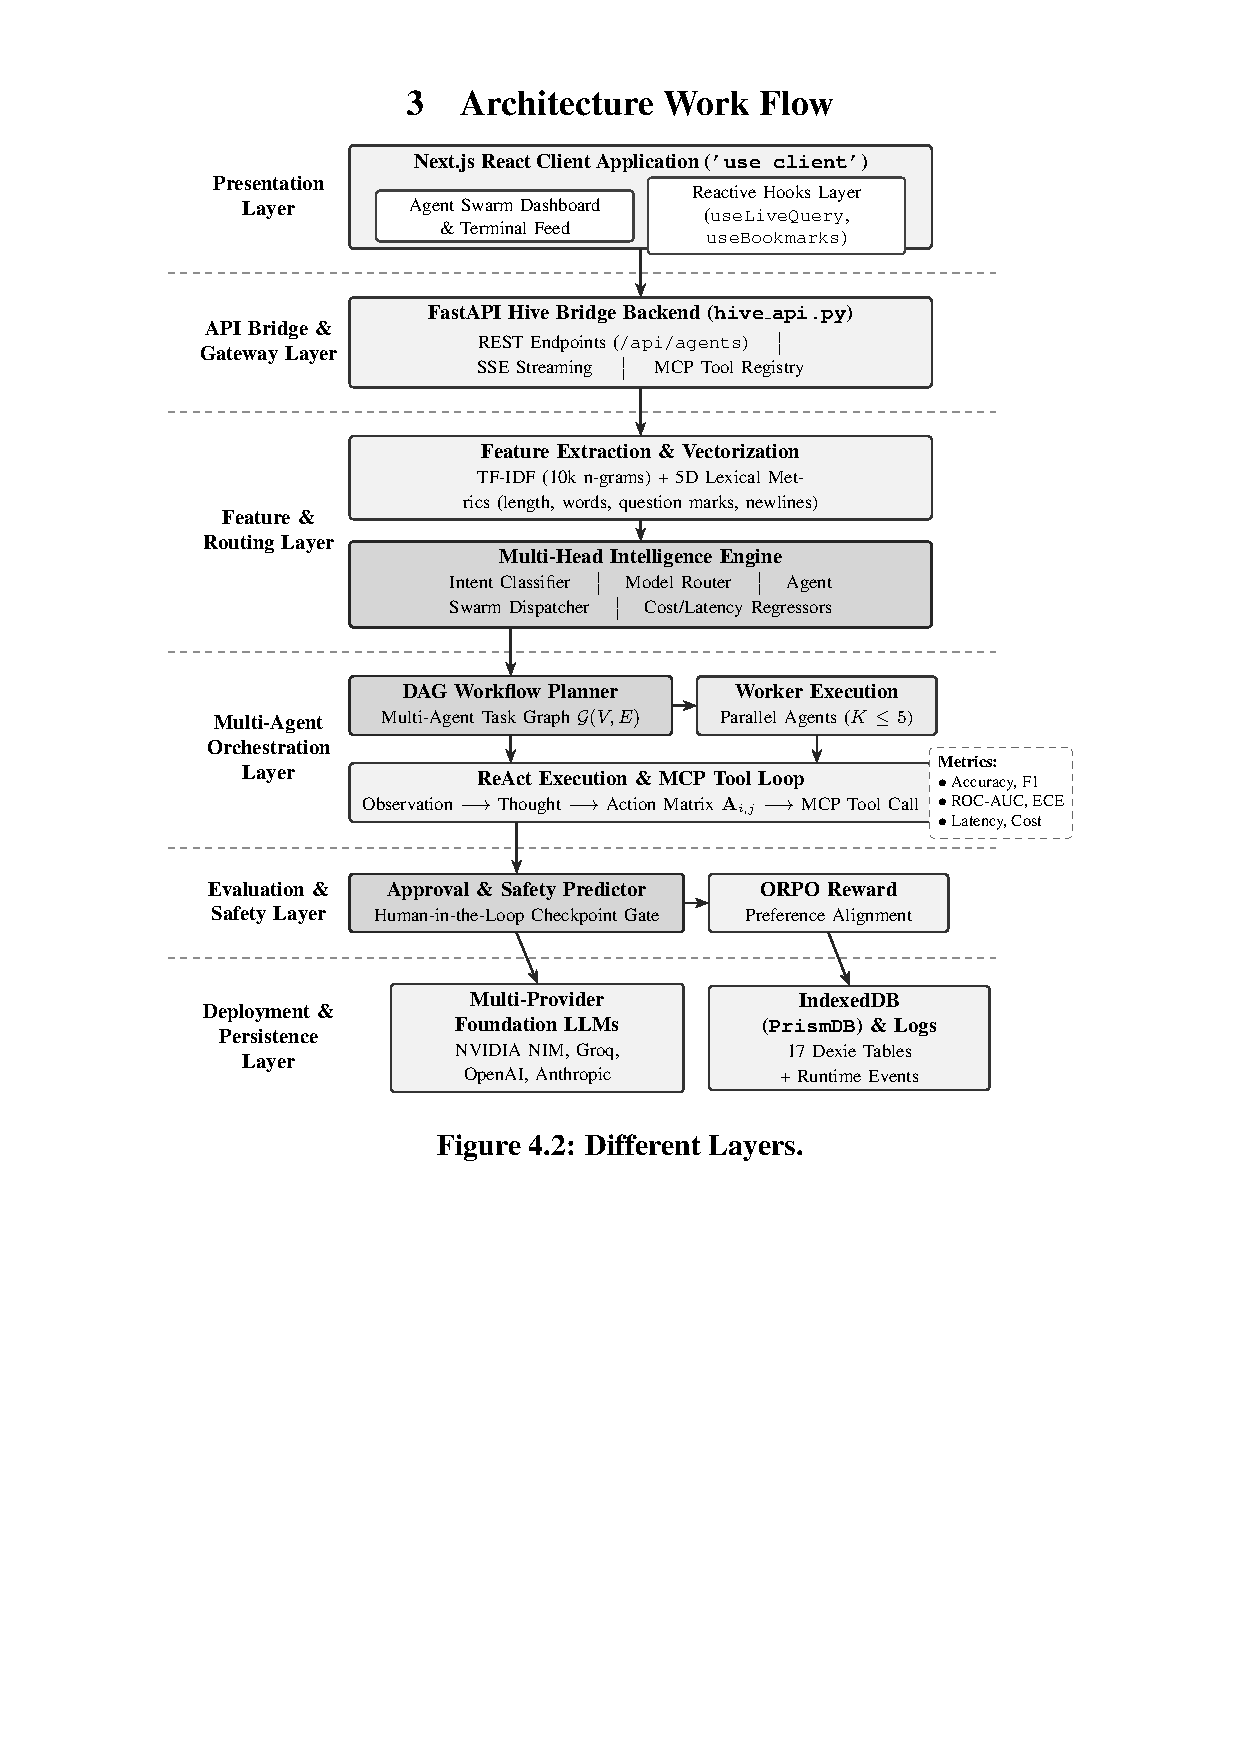
\includepdf[pages=1, fitpaper=true]{architecture_workflow.pdf}

\newpage
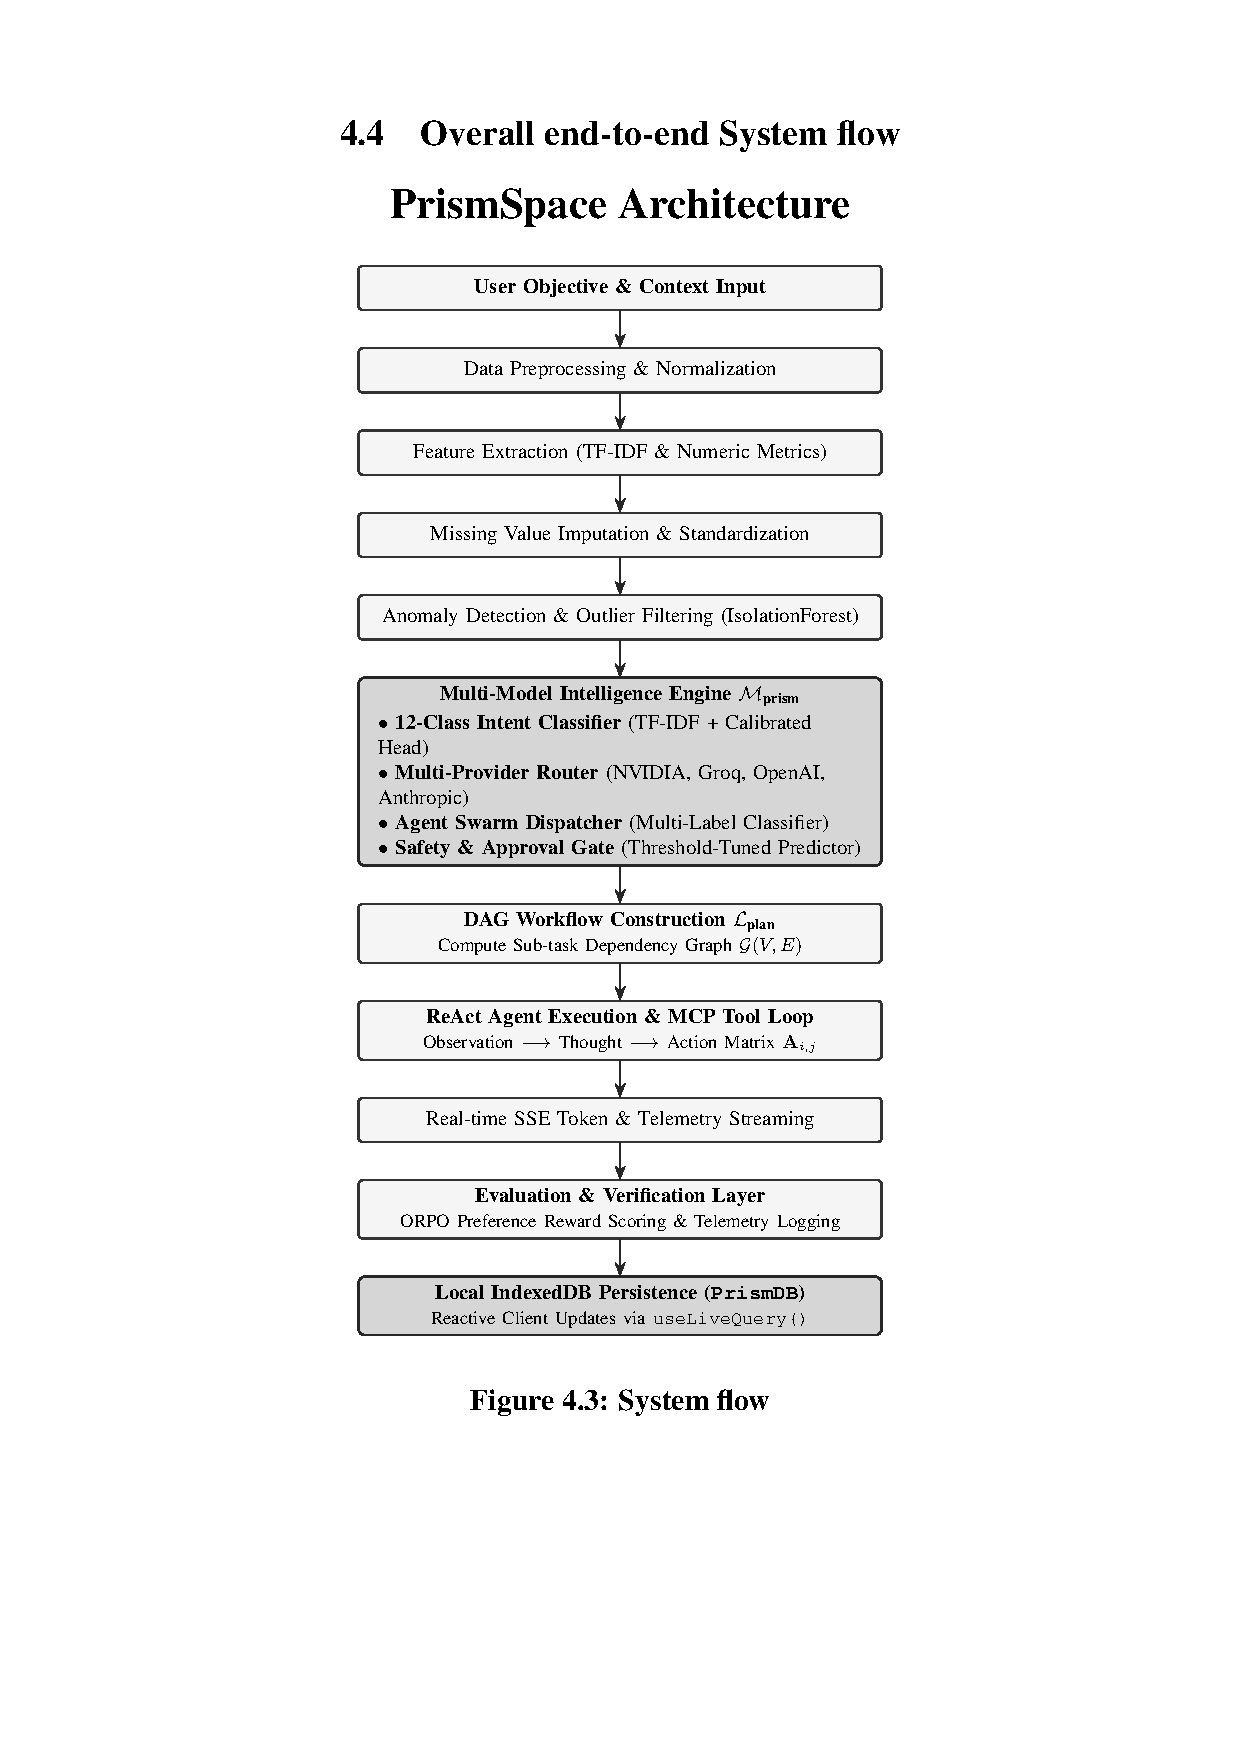
\includepdf[pages=1, fitpaper=true]{system_flow.pdf}

\newpage
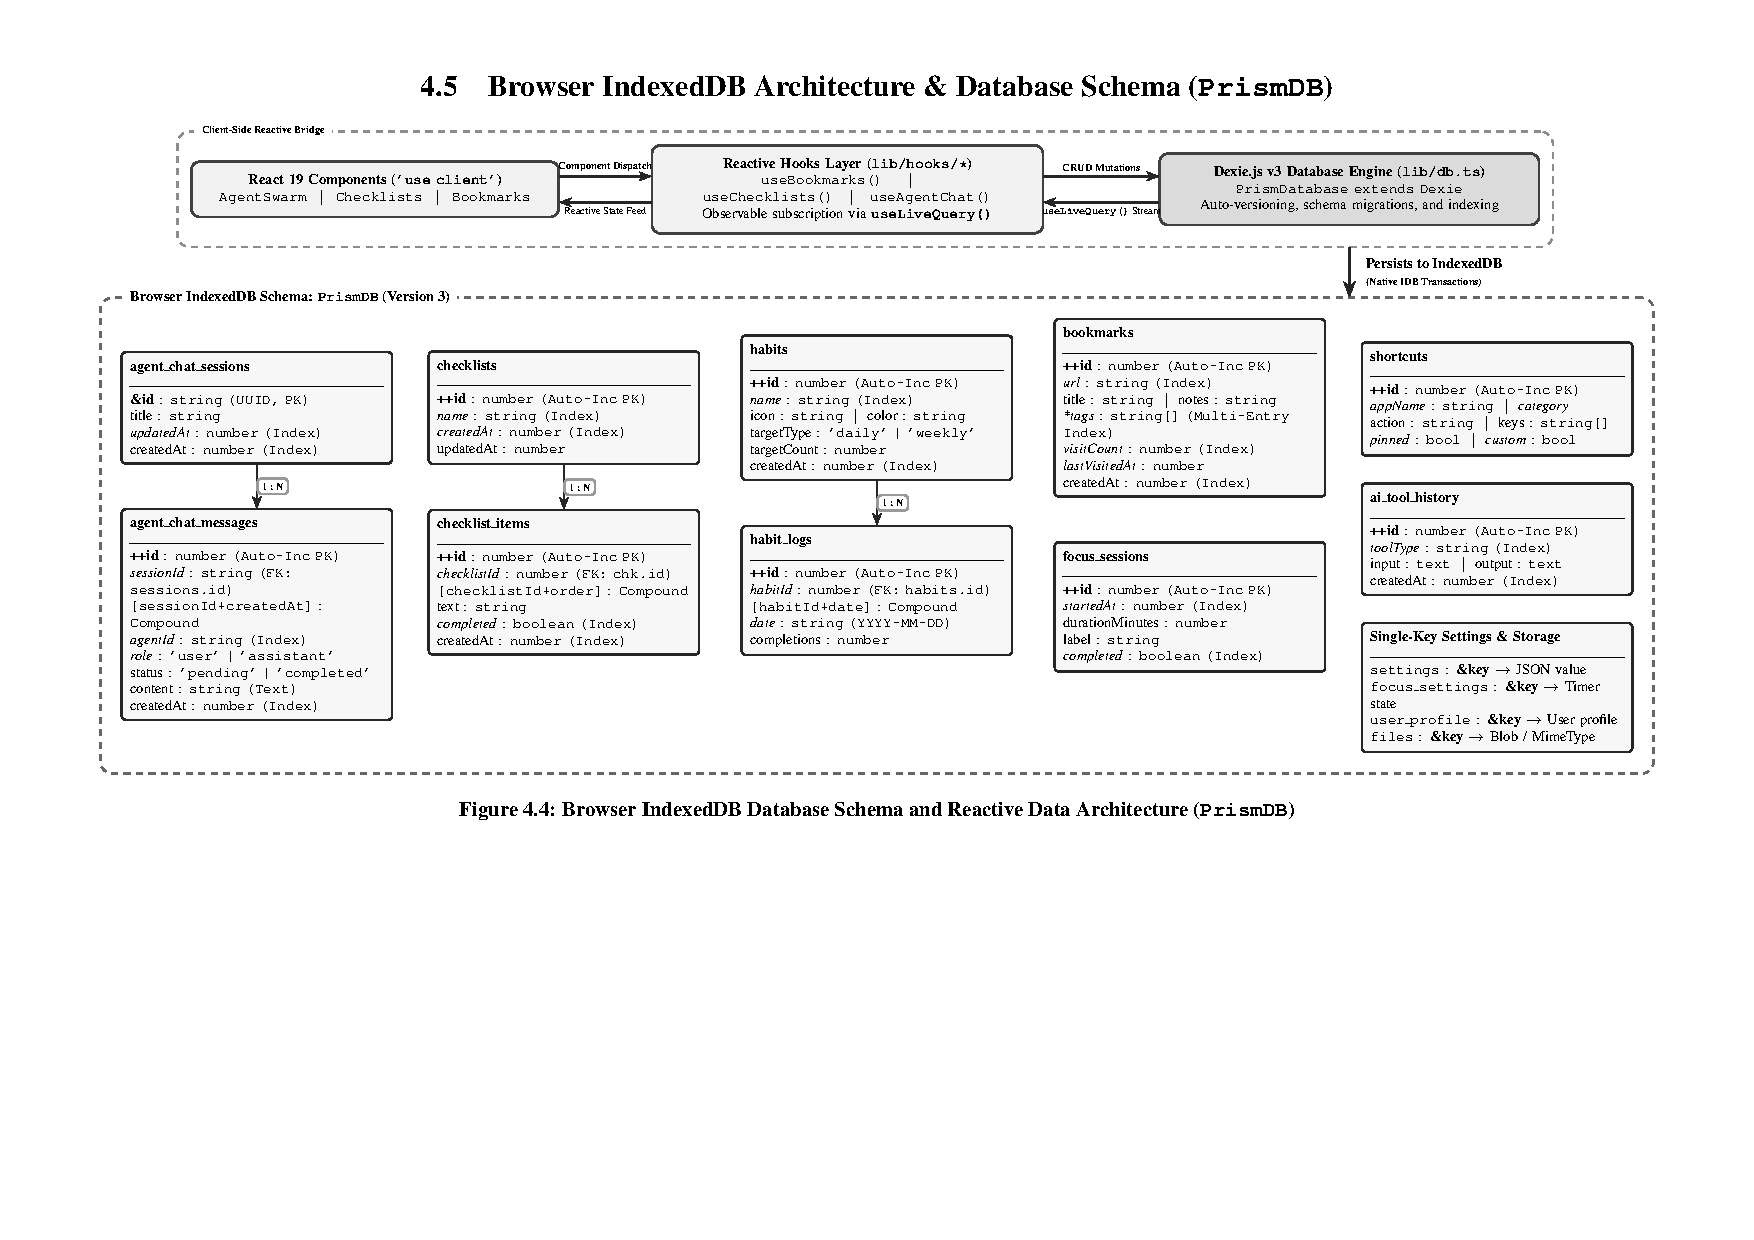
\includepdf[pages=1, fitpaper=true]{database_schema.pdf}

\newpage
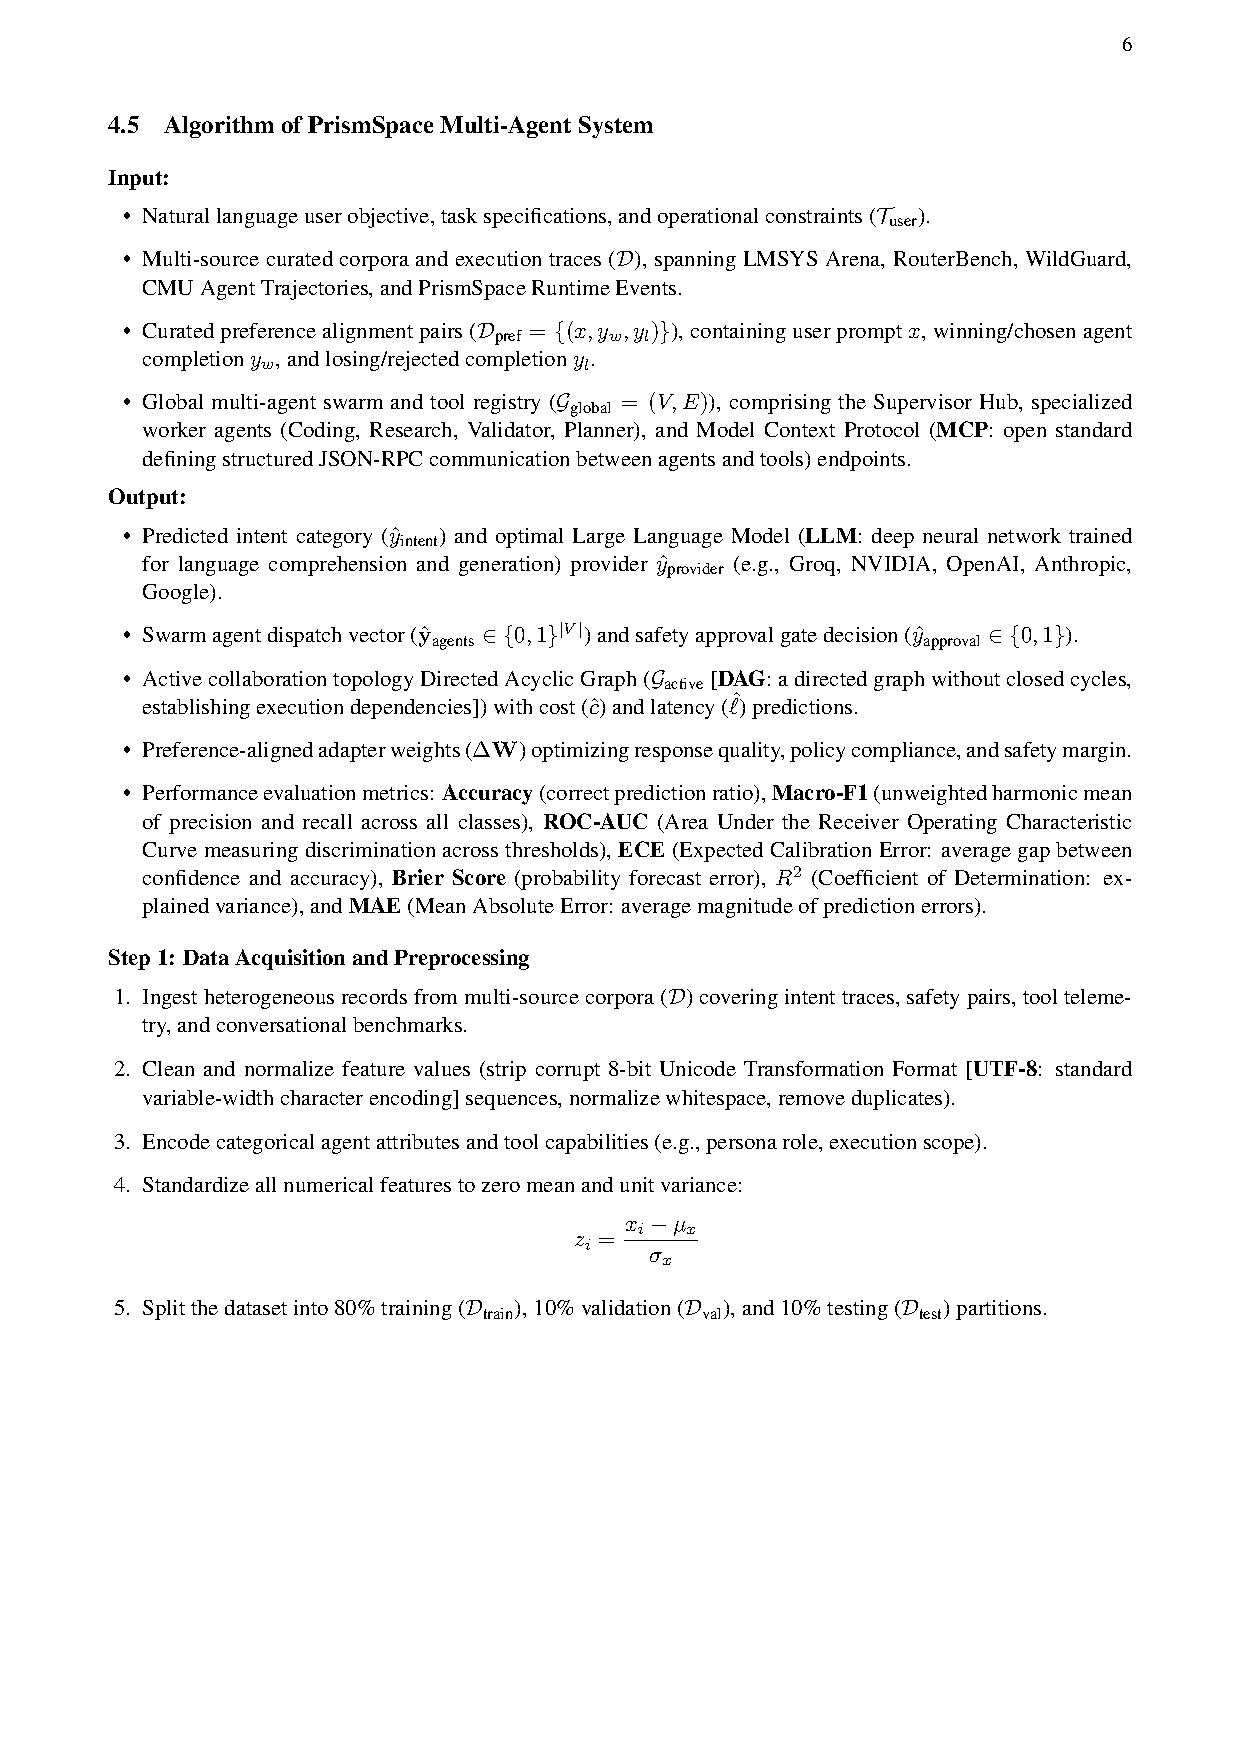
\includepdf[pages=-, fitpaper=true]{algorithm.pdf}

\end{document}
